\subsection{DevOps}\label{devops}

In der heutigen Gesellschaft gibt es zunehmend den Trend zu immer
schneller werdenden technologischen Entwicklungen und erhöhter Automatisierung. \footnote{Mazzara, vgl.~\cite{Mazzara2019}~[S.100]}

DevOps erfordert eine verstärkte Zusammenarbeit der an der Entwicklung und dem Betrieb beteiligten Teams.
\footnote{Kasteleiner/Schwartz, vgl.~\cite{Kasteleiner2019}~[S.211-214]}
\footnote{Siebra et. al, vgl.~\cite{Siebra2019}~[S.427]} \\

Die Abteilungen Development (Entwicklung) und Operations (Betrieb) haben in dem \textsl{klassischen Modell} unterschiedliche Ziele.
Die Entwicklungsabteilung will Software verändern und neue Funktionalitäten erstellen,
wo hingegen die Betriebsabteilung um Stabilität bemüht ist und jede Veränderung von Systemen als Risiko sieht.
DevOps soll diesen Konflikt durch Automatisierung, Tools und Praktiken auflösen.
Am Ende der Transformation soll ein reibungsarmer, sicherer und flüssiger Übergang der entwickelten Software in den Betrieb ermöglicht werden.
\footnote{Artac/Nitto, vgl.~\cite{Artac2017}~[S.497]} \\

Software Entwicklungsprozesse bei denen komplexe Übergaben an andere Teams erforderlich sind, schlagen eher fehl als optimierte Prozesse.
Übergaben werden durch Automatisierung und einfachere Kommunikation besser und sicherer. \footnote{Ozkaya, vgl.~\cite{Ozkaya2019}~[S.5]}
Die Auflösung von Silos, also eigenständigen Abteilungen, die nicht das große Ganze im Blick haben, ist hierfür erforderlich.
Dabei hat sich gezeigt, dass ein stabiler und risikoarmer Betrieb von Software bei hoher Änderungsrate nach der Auflösung solcher Silos vereinfacht wird.
\footnote{Samulat, vgl.~\cite{Samulat2017}~[S.205]} \\

Dabei geht es vor allem um eine kulturelle Veränderung im Unternehmen
mit dem Ziel, Hypothesen schneller am Markt testen zu können.
Kleine unabhängige Teams stehen im Vordergrund. \footnote{Kim et al, vgl.~\cite{Kim2018}}
Diese Teams sind sowohl für die Entwicklung als auch für den Betrieb der von ihnen erstellten Software zuständig.
Daraus ergibt sich, dass diese Teams vielfältiges Wissen über verschiedene Bereiche besitzen müssen.
\footnote{Wiedemann, vgl.~\cite{Wiedemann2019}~[S.157]} \\

\newpage

Jez Humble, einer der Vordenker der Bewegung, schrieb dazu:

\begin{quotation}
\textsl{DevOps, a movement of people who care about developing and operating reliable secure, high performance systems at scale.}
\footnote{König/Kugel, vgl.~\cite{Konig2019}~[S.291]}
\end{quotation}

Um den Begriff zu verdeutlichen, wird der unten abgebildete Zyklus verwendet.
Dieser Zyklus findet kontinuierlich statt und verfolgt das Ziel, die Zeit von der Idee bis zur Veröffentlichung an den Kunden zu optimieren.
Durch Monitoring und Feedback soll sichergestellt werden, dass die Entwicklung stets ausgerichtet an den Anforderungen stattfindet.
\footnote{Kasteleiner/Schwartz, vgl.~\cite{Kasteleiner2019}~[S.211-214]}

\begin{figure}[htb]
    \centering
    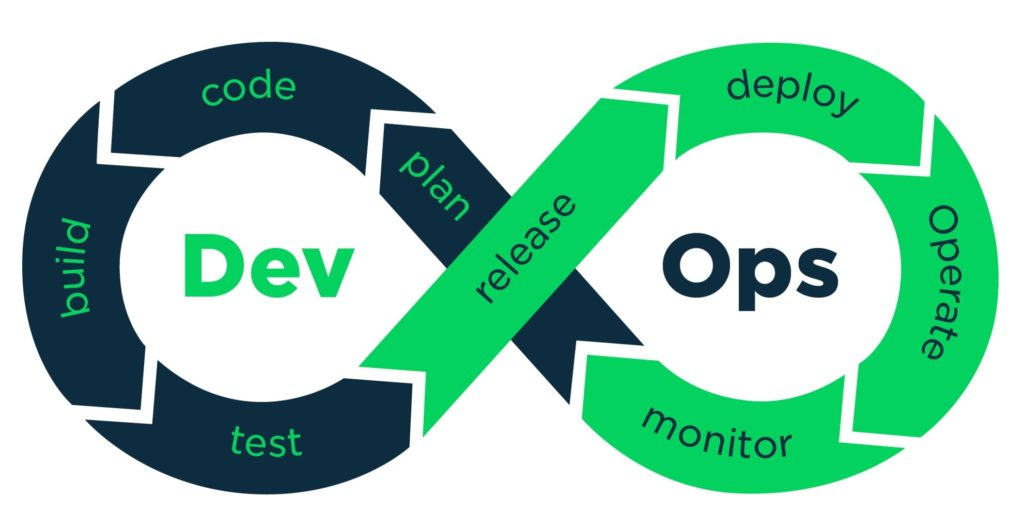
\includegraphics[width=0.6\textwidth]{images/devops_zyklus}
    \caption[DevOps Zyklus]{DevOps Zyklus \footnotemark}
    \label{fig:devops_zyklus}
\end{figure}
\footnotetext{Bildquelle: https://www.mt-ag.com/blog/know-how/devops/mit-jenkins-in-richtung-devops/}

DevOps beschreibt also keine Rolle, Team oder Abteilung und kann somit nicht eingestellt oder gekauft werden.
\footnote{König/Kugel, vgl.~\cite{Konig2019}~[S.292]}
Es geht dabei um mehr als nur um Automatisierung und Infrastructure as Code.
\footnote{Lichtenberger, vgl.~\cite{Lichtenberger2017}~[S.244]}

Die Auflösung von Silos soll die Entwicklung von komplexen Produkten beschleunigen und sicherer machen.
In der Literatur wird hierzu das \textbf{CAMS Model} genannt:
\footnote{Kasteleiner/Schwartz, vgl.~\cite{Kasteleiner2019}~[S.211-214]}
\footnote{Mazzara, vgl.~\cite{Mazzara2019}~[S.104]}

\begin{itemize}
    \item \textbf{Culture:}
    Kultureller Wandel ist einer der wichtigsten Aspekte von DevOps.
    Dabei sind die Nutzung von Scrum, Auflösung von Silos und der Wille in die umfangreiche Investition in die Weiterentwicklung maßgebend.

    \item \textbf{Automation:}
    Automatisierung und Vermeidung von manuellen Übergabeprozessen ist notwendig, um den Informationsfluss zu beschleunigen und Fehler zu vermeiden.

    \item \textbf{Measurement:}
    Kontinuierliche Verbesserung stellt eine der Kernkomponenten dar.
    Durch Metriken können Verbesserungen festgestellt und Verbesserungspotenziale identifiziert werden.


    \item \textbf{Sharing:}
    Transparenz und Wissenstransfer sind notwendig, um ein gemeinsames Wissen zu schaffen.
\end{itemize}

%Die Literatur benennt noch weitere Kombinationen dieses Kunstworts.
%Das wird häufig auch als StarOps bezeichnet zusätzliche Bezeichnungen sind hier:
%ArchOps, BizDevOps, SecDevOps, NoOps, AgileOps.
%\footnote{König/Kugel, vgl.~\cite{Konig2019}~[S.292]}


%    [RESTE]
%    X Testing hypotheses, organizational success is a common goal, reduce fricton, small independent teams deliver sw with self service tools, quick, safe and reliable, maximize developer productivity `(Kim et al)`
%    X Auflösung von Silos `(Schwarz/Kasteleiner)`
%    - DevOps is a recent approach that intends to improve the collaboration between development and IT operations teams, in order to establish a continuous and efficient deployment process. `(Siebra, 427)`
%    - a  set  of  practices  intended  to  reduce  the  time  between  committing  a  change  to  a  system  and  the  change  being  placed  into normal production, while ensur-ing  high  quality. `(Ozkaya, 3)`
%    - DevOps ist mehr => Lernzyklus beschleunigen, Zusammenarbeit der Fachabteilungen `(Schwarz/Kasteleiner)`
%    - DevOps as a concept for integrating the tasks, knowledge, and skills pertaining to the planning, building, and running of activities in a single cross- functional team that is responsible for the combined development and operational tasks of one or more software service products `(Wiedemann, 157)`
%    X Voraussetzung für DevOps: Automatisierte Prozesse in hoher Qualität und minimale Übergaben `(Schwarz/Kasteleiner)`
%    X Individual Software als Hauptprodukt eines Unternehmens `(Schwarz/Kasteleiner)`
%    X DevOps entails a series of socio-technical and organizational practices and tools that address and tackle these distances one by one until a frictionless, fluent, and resilient organization is distilled. (use of the same knowledge-base) `(Artac, Nitto, P. 497)`
%    - Standardsoftware einmal gekauft, Verbesserungen automatisch `(Schwarz/Kasteleiner, 1ff)`
%    X DevOps ist keine Rolle, Team, Abteilung, Toolchain Prüfsiegel oder Regulierung die eingestellt, gekauft oder erfüllt werden kann. `(König/Kugel, P. 292)`
%    X Software development processes  that  replace  communica-tion  with  over-the-wall  tasks  conse-quently  fail
